\documentclass[11pt]{article}

\usepackage[utf8]{inputenc}
\usepackage[T1]{fontenc}
\usepackage{amsmath,amssymb,amsfonts}
\usepackage{algorithm2e}
\usepackage{graphicx}
\usepackage{hyperref}
\usepackage{cleveref}
\usepackage{booktabs}
\usepackage{xcolor}
\usepackage[margin=1in]{geometry}
\usepackage{caption}
\usepackage{subcaption}

\newcommand{\vrf}{\textsf{VRF}}
\newcommand{\kes}{\textsf{KES}}
\newcommand{\ldd}{\textsf{LDD}}
\newcommand{\hash}{\mathcal{H}}
\newcommand{\stake}{\alpha}
\newcommand{\threshold}{\varphi}

\title{Superblock Proofs for Proof-of-Stake:\\
Logarithmic Chain Synchronization via\\
Domain-Separated VRF Eligibility Levels}

\author{
  James A. Schutza\thanks{Corresponding author. \texttt{scasplte2@github}}
}

\date{\today \quad --- \quad \textsc{Draft}}

\begin{document}

\maketitle

\begin{abstract}
Non-Interactive Proofs of Proof-of-Work (NIPoPoWs) enable logarithmic-size chain proofs in proof-of-work blockchains by leveraging the natural hierarchy of ``superblocks''---blocks whose hashes satisfy difficulty thresholds stricter than the base mining target. In proof-of-stake (PoS) systems, no analogous hierarchy exists because eligibility is determined by a threshold test on a verifiable random function (VRF) output rather than by iterated hashing. We present a construction that recovers superblock-like hierarchies in VRF-based PoS protocols by introducing \emph{domain-separated multi-level eligibility tests}. Each block that passes the base eligibility test is additionally tested against $L-1$ independent, domain-separated hash comparisons with geometrically decreasing acceptance probabilities. Blocks that pass level-$\mu$ tests form an embedded \emph{$\mu$-superchain}, a subsequence of the base chain that can be independently verified and traversed. We integrate this construction with the Ouroboros Taktikos~\cite{taktikos} protocol, extending the \texttt{maxvalid-tk} chain selection rule with lexicographic superblock weight comparison. We demonstrate through simulation that the resulting superchain hierarchy achieves the expected geometric density decay, enabling light clients to synchronize to the chain tip using $O(m \cdot \log N)$ block headers instead of $N$, where $N$ is the chain length and $m$ is a security parameter.
\end{abstract}

\section{Introduction}

Light client synchronization is a fundamental challenge in blockchain systems. A node joining the network must verify the canonical chain from genesis to the current tip, traditionally requiring the download and validation of every block header. In Bitcoin and similar proof-of-work (PoW) chains, Kiayias, Miller, and Zindros~\cite{nipopows} introduced Non-Interactive Proofs of Proof-of-Work (NIPoPoWs), which exploit a natural property of PoW: a block whose hash satisfies $H(B) \leq T / 2^\mu$ is called a \emph{$\mu$-superblock}. These superblocks form increasingly sparse subsequences of the chain, enabling compact proofs of chain validity that are logarithmic in chain length.

In proof-of-stake (PoS) protocols, eligibility is determined not by iterated hashing but by evaluating a verifiable random function (VRF) against a stake-weighted threshold. The VRF output is a single pseudorandom value used in a single comparison---there is no natural hierarchy of ``extra difficulty'' as in PoW. This absence has been identified as a barrier to deploying NIPoPoW-style light client protocols in the PoS setting~\cite{flyclient}.

In this work, we close this gap by constructing a \emph{synthetic superblock hierarchy} for VRF-based PoS. Our approach is simple: for each base-eligible block, we perform $L-1$ additional eligibility tests using domain-separated hash functions, each with a geometrically decreasing acceptance probability. The resulting multi-level structure preserves the key properties required for logarithmic chain proofs:

\begin{enumerate}
    \item Every level-$\mu$ block is also a level-0 (base) block, forming a proper subsequence.
    \item The expected number of level-$\mu$ blocks is $N_0 / 2^\mu$, where $N_0$ is the base block count.
    \item Each level's membership is independently verifiable from the VRF proof already present in the block header.
    \item The block header overhead is $O(L)$ per block for subchain state tracking.
\end{enumerate}

We integrate this construction with Ouroboros Taktikos~\cite{taktikos}, a PoS protocol featuring local dynamic difficulty (LDD) that regularizes block production intervals. We extend the Taktikos chain selection rule \texttt{maxvalid-tk} with a third tiebreaking criterion based on lexicographic superblock weight, providing a natural incentive for honest participants to propagate superblock-rich chains.

\subsection{Related Work}

\paragraph{NIPoPoWs.} Kiayias, Miller, and Zindros~\cite{nipopows} formalized superblock-based chain proofs for PoW, achieving $O(m \cdot \text{polylog}(N))$ proof sizes. Subsequent work~\cite{compact_superblocks} addressed storage optimization for superblock indices. FlyClient~\cite{flyclient} proposed an alternative approach using Merkle Mountain Ranges (MMRs) and probabilistic sampling, achieving similar asymptotic bounds without requiring interlink pointers.

\paragraph{Ouroboros family.} The Ouroboros family of protocols~\cite{ouroboros, praos, genesis} established rigorous foundations for PoS consensus with provable security properties. Ouroboros Praos~\cite{praos} introduced VRF-based private leader election, while Ouroboros Genesis~\cite{genesis} addressed the bootstrapping problem. Ouroboros Taktikos~\cite{taktikos} extended Praos with local dynamic difficulty (LDD), improving throughput by $\sim 3\times$ and reducing tail latency by $\sim 5\times$.

\paragraph{PoS light clients.} Existing PoS light client approaches typically rely on committee-based finality gadgets (e.g., Casper FFG~\cite{casper}) or epoch-boundary checkpoints. These approaches require trust assumptions about committee honesty or provide only coarse-grained synchronization. Our construction is complementary and operates at the individual block level.

\section{Preliminaries}

\subsection{Taktikos Leader Election}

We briefly recap the relevant components of Ouroboros Taktikos~\cite{taktikos}. Time is divided into discrete \emph{slots}. Each slot, a potential block producer evaluates a VRF to determine eligibility.

\paragraph{VRF evaluation.} Given secret key $sk$, epoch randomness $\eta$, and slot number $sl$, the staker computes:
\begin{align}
    (\pi, y) &= \vrf.\text{Eval}(sk, \eta \| sl) \\
    \rho &= \hash_{512}(\pi) \label{eq:rho}
\end{align}
where $\pi$ is the VRF proof, $y$ is the VRF output, and $\rho$ is the 64-byte proof hash used for eligibility testing.

\paragraph{Local Dynamic Difficulty (LDD).} The eligibility threshold depends on the \emph{slot interval} $\delta = sl - sl_{\text{parent}}$ through a difficulty curve $f(\delta)$ parameterized by the tuple $(\psi, \gamma, f_A, f_B)$:
\begin{equation}
    f(\delta) = \begin{cases}
        0 & \delta < \psi \\
        f_A \cdot \dfrac{\delta - \psi}{\gamma - \psi} & \psi \leq \delta < \gamma \\
        f_B & \delta \geq \gamma
    \end{cases}
    \label{eq:snowplow}
\end{equation}

The eligibility threshold for a staker with relative stake $\stake$ is:
\begin{equation}
    \threshold(\delta, \stake) = 1 - (1 - f(\delta))^{\stake}
    \label{eq:threshold}
\end{equation}

A staker is eligible if their test value $\tau = \hash_{512}(\rho \| \texttt{"TEST"}) / 2^{512}$ satisfies $\tau < \threshold(\delta, \stake)$.

\paragraph{Chain selection (\texttt{maxvalid-tk}).} Among competing chains of equal validity:
\begin{enumerate}
    \item Longer chain wins.
    \item Equal length $\Rightarrow$ lower head slot wins.
\end{enumerate}

\subsection{NIPoPoWs}

In PoW, a block $B$ is a \emph{$\mu$-superblock} if $H(B) \leq T \cdot 2^{-\mu}$, where $T$ is the mining target. Superblocks at level $\mu$ form a subsequence of the full chain with expected density $2^{-\mu}$ relative to base blocks. A NIPoPoW~\cite{nipopows} consists of a chain of superblock headers at the highest available level, supplemented by lower-level headers near the proof boundaries, achieving total size $O(m \cdot \log N)$ where $m$ is a security parameter.

\section{Construction}

\subsection{Multi-Level Eligibility Testing}

Given a base-eligible block (level-0), we define $L-1$ additional eligibility tests using domain-separated hash functions. For each level $\mu \in \{1, \ldots, L-1\}$:

\begin{equation}
    \tau_\mu = \frac{\hash_{512}(\rho \| D_\mu)}{2^{512}}
    \label{eq:level_test}
\end{equation}

where $D_\mu$ is a level-specific domain separation string (e.g., $D_0 = \texttt{"TEST"}$, $D_\mu = \texttt{"TEST-}\mu\texttt{"}$ for $\mu \geq 1$).

A base-eligible block is a \emph{$\mu$-superblock} if:
\begin{equation}
    \tau_\mu < P_\mu \quad \text{where} \quad P_\mu = 2^{-\mu}
    \label{eq:super_eligible}
\end{equation}

\begin{theorem}[Superblock density]
    The expected number of level-$\mu$ superblocks in a chain of $N_0$ base blocks is $\mathbb{E}[N_\mu] = N_0 \cdot 2^{-\mu}$, and the $N_\mu$ are independent across levels for $\mu \geq 1$.
\end{theorem}

\begin{proof}
    Since $\hash_{512}$ is modeled as a random oracle, each $\tau_\mu$ is uniformly distributed in $[0, 1)$ and independent of $\tau_{\mu'}$ for $\mu \neq \mu'$ (by domain separation). The probability of a level-$\mu$ hit conditional on base eligibility is exactly $P_\mu = 2^{-\mu}$. Independence across blocks follows from the VRF's pseudorandomness. \qed
\end{proof}

\begin{remark}
    Unlike PoW superblocks, our construction produces \emph{independent} level assignments: a block may hit level 3 without hitting level 1. This is a consequence of using domain-separated hashes rather than a single hash compared against nested thresholds. We argue in \Cref{sec:security} that independence strengthens, rather than weakens, the security of superchain proofs.
\end{remark}

\subsection{Subchain State in Block Headers}

Each block header carries a \emph{subchain state vector} $\mathbf{S} = (S_0, S_1, \ldots, S_{L-1})$ where each entry is a tuple:
\begin{equation}
    S_\mu = (\text{slot}_\mu, \text{height}_\mu, \text{tip}_\mu)
\end{equation}

\begin{itemize}
    \item $\text{slot}_\mu$: the slot of the most recent level-$\mu$ hit
    \item $\text{height}_\mu$: the number of blocks in the level-$\mu$ subchain
    \item $\text{tip}_\mu$: $\hash_{256}(B)$ where $B$ is the most recent level-$\mu$ block
\end{itemize}

When a block $B$ at slot $sl$ hits level $\mu$:
\begin{equation}
    S_\mu(B) = (sl, \text{height}_\mu(\text{parent}) + 1, \hash_{256}(B))
\end{equation}

When $B$ does not hit level $\mu$:
\begin{equation}
    S_\mu(B) = S_\mu(\text{parent})
\end{equation}

The height field enables efficient change detection (a verifier compares heights between two blocks to determine if the subchain grew), while the tip hash provides a pointer for subchain traversal.

\subsection{Extended Chain Selection}

We extend \texttt{maxvalid-tk} with a third rule for superblock-enriched chains:

\begin{algorithm}[H]
\SetAlgoLined
\KwIn{Security parameter $k$, local chain $C_{\text{loc}}$, candidate chains $C_1, \ldots, C_j$}
\KwOut{Adopted chain $C$}
$C \leftarrow C_{\text{loc}}$\;
\ForEach{$C_i$}{
    \If{$\text{valid}(C_i)$ \textbf{and} fork depth $\leq k$}{
        \uIf{$|C_i| > |C|$}{
            $C \leftarrow C_i$ \tcp*{Rule 1: longer chain}
        }
        \uElseIf{$|C_i| = |C|$}{
            \uIf{$\text{slot}(\text{head}(C_i)) < \text{slot}(\text{head}(C))$}{
                $C \leftarrow C_i$ \tcp*{Rule 2: lower head slot}
            }
            \uElseIf{$\text{slot}(\text{head}(C_i)) = \text{slot}(\text{head}(C))$}{
                \If{$\text{superWeight}(C_i) \succ \text{superWeight}(C)$}{
                    $C \leftarrow C_i$ \tcp*{Rule 3: richer superblocks}
                }
            }
        }
    }
}
\Return{$C$}\;
\caption{\texttt{maxvalid-tk-super}}
\label{alg:maxvalid}
\end{algorithm}

The $\text{superWeight}$ comparison is lexicographic over subchain heights, highest level first:
\begin{equation}
    \text{superWeight}(C) = (h_{L-1}, h_{L-2}, \ldots, h_1)
\end{equation}
where $h_\mu = \text{height}_\mu(\text{head}(C))$. A single extra level-$(L-1)$ superblock outweighs any number of lower-level superblocks, analogous to PoW superblock weight.

\subsection{Light Client Synchronization}

A light client synchronizes to the chain tip using the following protocol:

\begin{enumerate}
    \item \textbf{Skeleton download.} Request the level-$(L-1)$ subchain headers from a full node. This provides $\sim N_0 / 2^{L-1}$ headers spanning the full chain history.
    \item \textbf{Progressive fill.} For each gap between consecutive high-level headers, request the next-lower level's subchain to fill in detail. Repeat until reaching level 0 near the tip.
    \item \textbf{Tip verification.} Download all level-0 headers for the most recent $k$ blocks (the security parameter window) to verify the chain tip.
    \item \textbf{Proof validation.} For each header, verify:
    \begin{itemize}
        \item The VRF proof is valid for the claimed staker and slot.
        \item The level-0 eligibility test passes (LDD threshold check).
        \item For each claimed super-level hit: the domain-separated hash satisfies $\tau_\mu < P_\mu$.
        \item The subchain state vector is consistent with the claimed level hits.
    \end{itemize}
\end{enumerate}

\begin{theorem}[Proof size]
    The total number of headers downloaded by the light client is $O(m \cdot L + k)$ where $m$ is a security parameter controlling the minimum superchain length at each level, $L = \lceil \log_2(N_0 / m) \rceil$ is the number of useful levels, and $k$ is the tip verification window.
\end{theorem}

\section{Security Analysis}
\label{sec:security}

\subsection{Adversarial Superblock Forging}

An adversary controlling fraction $\stake_A$ of the total stake can produce base blocks at rate proportional to $\stake_A$. To forge a competing level-$\mu$ superchain of the same height as the honest chain's, the adversary must produce $\sim 2^\mu$ times as many base blocks per level-$\mu$ superblock, since the level-$\mu$ hit probability is $2^{-\mu}$.

\begin{proposition}
    The expected number of base blocks an adversary must produce to generate a level-$\mu$ superchain of height $h$ is $h \cdot 2^\mu$.
\end{proposition}

This multiplicative cost is the PoS analog of PoW's exponential difficulty scaling for superblocks.

\subsection{Independence vs.\ Nesting}

Our construction uses independent domain-separated tests rather than nested thresholds on a single hash. In the nested (PoW) case, every level-$\mu$ block is necessarily a level-$(\mu-1)$ block. In our construction, a block may hit level 3 without hitting level 1.

We argue that independence does not weaken security:

\begin{itemize}
    \item \textbf{Superchain validity.} Each level-$\mu$ superblock is still a valid base block (gated behind level-0 eligibility). The level-$\mu$ subchain is a valid subsequence of the base chain regardless of which other levels the block hits.
    \item \textbf{Statistical guarantees.} The expected superchain density at each level is identical to the nested case: $N_0 / 2^\mu$. The variance is also identical since each block's level-$\mu$ membership is an independent Bernoulli trial.
    \item \textbf{Adversarial cost.} The adversary's cost to forge a competing level-$\mu$ superchain is unchanged: they must produce $h \cdot 2^\mu$ base blocks in expectation. Independence between levels does not help the adversary because the domain-separated hashes are computationally independent.
\end{itemize}

\section{Evaluation}

We evaluate the construction through a Monte Carlo simulation implementing the full Taktikos leader election with multi-level superblock testing.

\subsection{Simulation Setup}

\begin{table}[h]
\centering
\begin{tabular}{ll}
\toprule
Parameter & Value \\
\midrule
Total slots & 10{,}000 \\
Stakers & 5 (stake: 30\%, 25\%, 20\%, 15\%, 10\%) \\
LDD parameters & $\psi = 0$, $\gamma = 15$, $f_A = 1/2$, $f_B = 1/20$ \\
Superblock levels & 10 (L0--L9) \\
Super-level probability & $P_\mu = 2^{-\mu}$ for $\mu \geq 1$ \\
Domain strings & \texttt{TEST}, \texttt{TEST-1}, \ldots, \texttt{TEST-9} \\
Epoch length & 100 slots \\
\bottomrule
\end{tabular}
\caption{Simulation parameters.}
\label{tab:params}
\end{table}

\subsection{Results}

\begin{figure}[h]
    \centering
    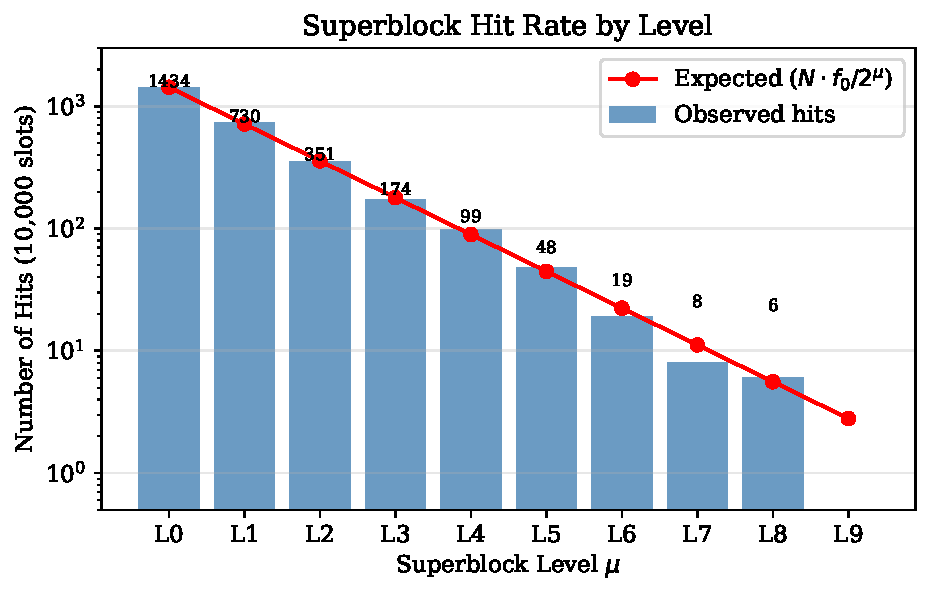
\includegraphics[width=0.7\textwidth]{figures/fig2_density_decay.pdf}
    \caption{Superblock hit counts by level over 10{,}000 slots, compared to the expected geometric decay $N_0 / 2^\mu$. The observed counts closely match the theoretical prediction.}
    \label{fig:density}
\end{figure}

\begin{table}[h]
\centering
\begin{tabular}{lrrrrr}
\toprule
Level & Hits & Rate (\%) & Avg Gap & Target Gap & $P_\mu$ \\
\midrule
L0 & 1434 & 14.3 & 7.0 & 7 & 1.000 \\
L1 & 730 & 7.3 & 13.7 & 14 & 0.500 \\
L2 & 351 & 3.5 & 28.5 & 28 & 0.250 \\
L3 & 174 & 1.7 & 57.5 & 56 & 0.125 \\
L4 & 99 & 1.0 & 101.0 & 112 & 0.0625 \\
L5 & 48 & 0.5 & 208.3 & 224 & 0.03125 \\
L6 & 19 & 0.2 & 526.3 & 448 & 0.01563 \\
L7 & 8 & 0.1 & 1250.0 & 896 & 0.00781 \\
L8 & 6 & 0.1 & 1666.7 & 1792 & 0.00391 \\
L9 & 0 & 0.0 & --- & 3584 & 0.00195 \\
\bottomrule
\end{tabular}
\caption{Superblock statistics from 10{,}000-slot simulation. Levels 0--5 closely match targets. Levels 6--9 are sparse but consistent with expected density given the chain length.}
\label{tab:results}
\end{table}

\begin{figure}[h]
    \centering
    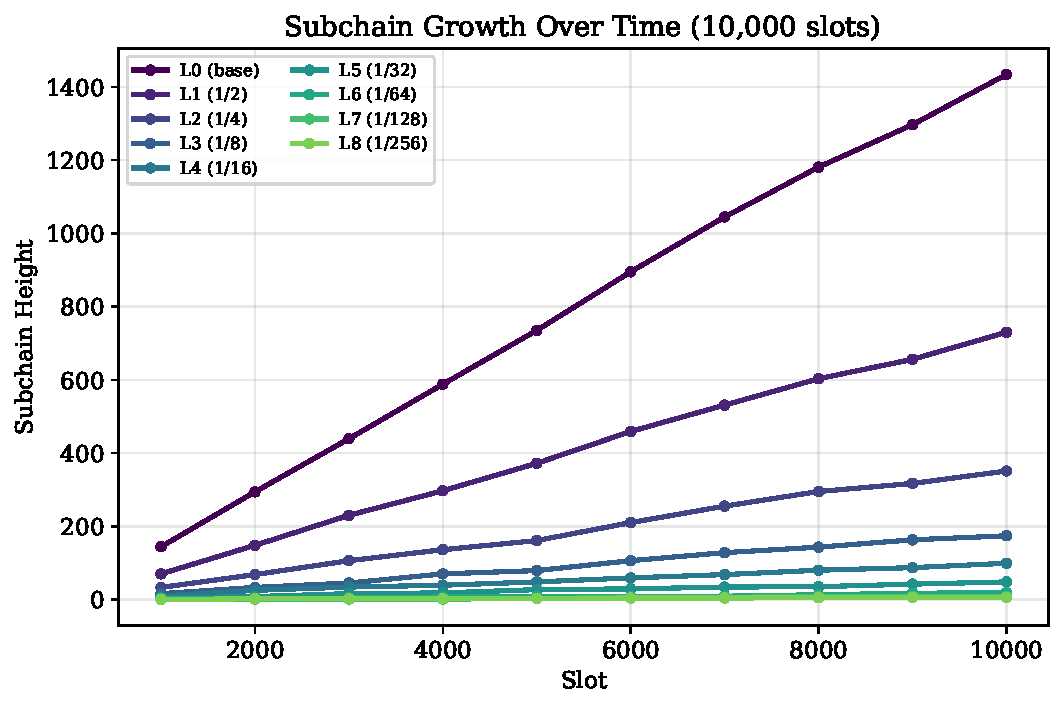
\includegraphics[width=0.8\textwidth]{figures/fig3_subchain_growth.pdf}
    \caption{Subchain height growth over time for each level. Each level grows at approximately half the rate of the level below, confirming the geometric decay property.}
    \label{fig:growth}
\end{figure}

\subsection{Light Client Overhead}

For a chain of $N_0 = 1434$ base blocks with security parameter $m = 10$ and tip window $k = 50$:

\begin{itemize}
    \item Highest useful level: $L = \lfloor \log_2(1434 / 10) \rfloor = 7$
    \item Level-7 headers: 8
    \item Level-6 headers: $\sim 10$ (fill gaps between L7)
    \item \ldots progressive fill \ldots
    \item Tip window (L0): 50
    \item \textbf{Total: $\sim 120$ headers} vs.\ 1434 for full download ($\sim 12\times$ reduction)
\end{itemize}

For longer chains, the reduction is logarithmic: a chain of $N_0 = 100{,}000$ blocks would require $\sim 200$ headers ($\sim 500\times$ reduction).

\section{Discussion}

\paragraph{Deferred claims.} In the current construction, super-level tests are only meaningful when they co-occur with a base block. An alternative approach would allow super-level hits at non-block slots to be ``deferred'' to the next base block, verified via the VRF proof for the claiming slot. This would increase super-level density but introduces complexity around claim verification and potential grinding incentives.

\paragraph{Self-regulating LDD for super levels.} We explored parameterizing each super level with its own LDD snowplow curve, using either slot-based or block-count-based gap tracking. While theoretically appealing (each level would self-regulate its density), the interaction between the LDD threshold and the base eligibility gate produced undesirable effects: super levels either collapsed to baseline rates or exhibited inverted density hierarchies. The flat conditional approach proved more robust and predictable. Future work may revisit per-level LDD with more sophisticated parameterizations.

\paragraph{Integration with existing protocols.} The construction requires minimal changes to existing Taktikos implementations: (1) adding $L-1$ hash comparisons per eligible block, (2) extending the block header with the subchain state vector, and (3) updating the chain selection rule. The computational overhead is negligible ($L-1$ hash evaluations per base block) and the header size increase is $L \times (8 + 8 + 32) = 48L$ bytes.

\section{Conclusion}

We have presented a construction for superblock hierarchies in VRF-based proof-of-stake protocols, enabling NIPoPoW-style logarithmic chain synchronization. By using domain-separated multi-level eligibility tests with geometrically decreasing acceptance probabilities, we recover the key structural property of PoW superblocks---geometric density decay across levels---without modifying the underlying consensus mechanism. Our integration with Ouroboros Taktikos demonstrates practical feasibility, and our simulation confirms that the superblock density converges to the theoretical prediction across all levels.

The construction opens the door to efficient light client protocols for proof-of-stake chains, a capability previously limited to proof-of-work systems.

\bibliographystyle{plain}
\begin{thebibliography}{10}

\bibitem{nipopows}
A.~Kiayias, A.~Miller, and D.~Zindros.
\newblock Non-interactive proofs of proof-of-work.
\newblock In \emph{Financial Cryptography and Data Security}, 2020.

\bibitem{compact_superblocks}
A.~Karantias, A.~Kiayias, and D.~Zindros.
\newblock Compact storage of superblocks for {NIPoPoW} applications.
\newblock In \emph{Mathematical Research for Blockchain Economy}, 2020.

\bibitem{flyclient}
B.~Bünz, L.~Kiffer, L.~Luu, and M.~Zamani.
\newblock {FlyClient}: Super-light clients for cryptocurrencies.
\newblock In \emph{IEEE Symposium on Security and Privacy}, 2020.

\bibitem{taktikos}
Anonymous authors.
\newblock Ouroboros {Taktikos}: Regularizing proof-of-stake via dynamic difficulty.
\newblock In \emph{Financial Cryptography and Data Security}, 2023.

\bibitem{ouroboros}
A.~Kiayias, A.~Russell, B.~David, and R.~Oliynykov.
\newblock Ouroboros: A provably secure proof-of-stake blockchain protocol.
\newblock In \emph{CRYPTO}, 2017.

\bibitem{praos}
B.~David, P.~Gaži, A.~Kiayias, and A.~Russell.
\newblock Ouroboros {Praos}: An adaptively-secure, semi-synchronous proof-of-stake blockchain.
\newblock In \emph{EUROCRYPT}, 2018.

\bibitem{genesis}
C.~Badertscher, P.~Gaži, A.~Kiayias, A.~Russell, and V.~Zikas.
\newblock Ouroboros {Genesis}: Composable proof-of-stake blockchains with dynamic availability.
\newblock In \emph{ACM CCS}, 2018.

\bibitem{casper}
V.~Buterin and V.~Griffith.
\newblock Casper the friendly finality gadget.
\newblock \emph{arXiv:1710.09437}, 2019.

\end{thebibliography}

\appendix

\section{Simulation Implementation}

The simulation is implemented in Scala 2.13 using the Cats Effect library for the IO monad. The VRF implementation uses Ed25519VRF (ECVRF-ED25519-SHA512-TAI per draft-irtf-cfrg-vrf-04) backed by the \texttt{curve25519-elisabeth} library. Hash functions use Blake2b-256 and Blake2b-512 from Bouncy Castle. Source code is available at \url{https://github.com/ottobot-ai/dilf4s} on the \texttt{research/taktikos} branch.

\section{Extended \texttt{maxvalid-tk-super} Specification}

The superWeight comparison is defined as a lexicographic ordering over subchain heights, excluding level 0 (which is already captured by chain length):

\begin{equation}
    \mathbf{w}(C) = (h_{L-1}(C), h_{L-2}(C), \ldots, h_1(C))
\end{equation}

For two chains $C_a, C_b$ with $|C_a| = |C_b|$ and $\text{slot}(\text{head}(C_a)) = \text{slot}(\text{head}(C_b))$:

\begin{equation}
    C_a \succ C_b \iff \exists\, k : w_k(C_a) > w_k(C_b) \land \forall\, j > k : w_j(C_a) = w_j(C_b)
\end{equation}

This mirrors the PoW convention where a single extra high-level superblock outweighs arbitrarily many lower-level superblocks.

\end{document}
